\documentclass[11pt]{report}
\usepackage[margin=0.5in]{geometry}
\usepackage{mathpazo}
\usepackage{amsmath}
\usepackage[colorlinks=true]{hyperref}
\usepackage{parskip}
\usepackage{tikz}
\usepackage{circuitikz}
\usepackage{caption}
\usepackage{amssymb}
\usepackage{subcaption}

\tikzstyle{Si}=[circle,draw=blue,fill=blue!50,thick]

% Make lists condensed %
\usepackage{enumitem}
\setlist{nosep}

\begin{document}

\setcounter{chapter}{-1}

\chapter{MOSFETs}

\section{Intrinsic Semiconductors}

\subsection{Silicon}
% TODO: draw silicon diagram

Silicon is a group IV element, so it forms a covalent bond with 4 neighbours. At 0 Kelvin, the bonds are intact and no electrons are available for conduction, so it is an insulator. At room temperature, some bonds break, freeing electrons. This also creates \textbf{holes} in equal proportion. \autoref{eqn:free-electron-density} gives the number of free electrons per unit volume as a function of temperature.


\begin{equation}
	\label{eqn:free-electron-density}
	n_i = BT^{\frac{3}{2}}e^{-\frac{E_g}{2kT}}
\end{equation}

\begin{itemize}
	\item $B$ is a material-dependent parameter
	\item $E_g$ is the bandgap energy (for Silicon, 1.12eV) - the minimum energy required to break a covalent bond
	\item $k$ is Boltzmann's constant
\end{itemize}

\subsection{Doped Semiconductors}

Adding Phosphorous to a Silicon network adds free electrons. This creates \textbf{n-type} silicon. Adding Boron adds free holes. This creates \textbf{p-type} silicon. The dopant carriers (electrons and holes) cause two types of current to flow:

\subsubsection{Drift Current}
Drift current begins to flow when an electrical field is applied (or, equivalently, a potential difference appears) to a piece of silicon. The velocity of the carriers is given by
\begin{align*}
		v_{\text{p-drift}} &= \mu_p E \\
		v_{\text{n-drift}} &= \mu_n E
\end{align*}

Where $\mu$ is the \textbf{mobility} of the type of carrier. In silicon, $\mu_p$ is typically \textbf{lower} than $\mu_n$


\subsubsection{Diffusion Current}
Diffusion current is a result of a non-uniform density of carriers (e.g. at the boundary of two different dopings of Silicon). This is a typical differential equation problem and the main result is that this causes some carriers to travel into the rest of the silicon and even out the distribution, though the rate decreases as the process continues.

\section{PN Junction}

\begin{center}
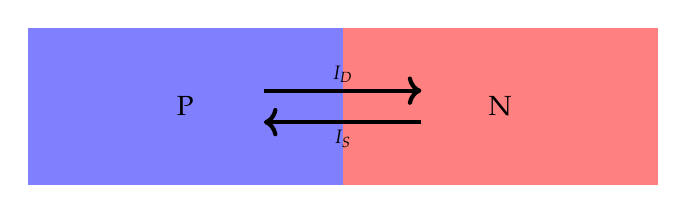
\begin{tikzpicture}[scale=4]
	\fill[blue!50] (0,0) rectangle (1, 0.5) node[pos=0.5,black]{P};
	\fill[red!50] (1,0) rectangle (2, 0.5)node[pos=0.5,black]{N};
	\draw [->, line width=1.5] (0.75, 0.3) -- (1.25,0.3) node[above,pos=0.5,black,scale=0.7]{$I_D$};
	\draw [->, line width=1.5] (1.25, 0.2) -- (0.75, 0.2) node[below, pos=0.5, black, scale=0.7]{$I_S$};
\end{tikzpicture}
\end{center}

In a PN junction, we have P-type silicon touching N-type silicon. The P-type silicon has free holes from doping, and some electrons from the intrinsic Silicon (depending on temperature). The N-type silicon has free electrons, and some holes from the intrinsic Silicon (depending again on the temperature). These are respectively the \textbf{majority} and \textbf{minority} carriers of each node. Recall that positive charges move towards a \textit{lower} potential (you can think of this as positive voltages \textit{repelling} positive charges.


\subsection{Diffusion Current}
As holes migrate from P to N due to diffusion, they neutralize some electrons. This \textit{uncovers} the minority carriers in N forming a slightly positive charged region in the N-type silicon near the boundary. The opposite process happens for electrons going from N to P which forms a \textbf{depletion region}. This forms a potential difference across the depletion region equal to the \textit{barrier voltage} $V_0$ that prevents more current from flowing from P to N.

\subsection{Drift Current}
Minority holes in the N-type silicon that drift towards the edge of the depletion region will be \textit{accelerated} by the potential drop towards the P-type silicon. The value of this current strongly depends on the temperature since that determines the density of minority carriers in each node.

\subsection{Equilibrium}
In equilibrium and open-circuit conditions, no current flows and thus $I_D = I_S$ which is maintained by the barrier voltage $V_0$. Thus, at room temperature we can experimentally determine $V_0$ for silicon as being in the range $0.6$V to $0.9$V

\subsection{Applied Voltage}
A PN junction is \textbf{reverse biased} when the net barrier voltage is positive. In this case, little to no current flows, except for a drift current that increases with the barrier voltage (as minority carriers are moved through more quickly in this case). A PN junction is \textbf{forward biased} when the applied voltage is negative. To maintain the applied voltage, there must be a source of electrons that tends to 'feed' the N-type silicon and thus drastically increases the \textbf{diffusion current}.

\subsection{Reverse Breakdown}
 At some point, a very negative positive barrier voltage will suddenly cause a huge current to flow from N to P. This is cause either by the \textbf{zener effect} or \textbf{avalanche effect}, the details of which are outside the scope of this course.


 \section{NMOS Transistors}

 The \textbf{N}-channel \textbf{M}etal-\textbf{O}xide-\textbf{S}emiconductor transistor has the following structure


 \begin{center}
 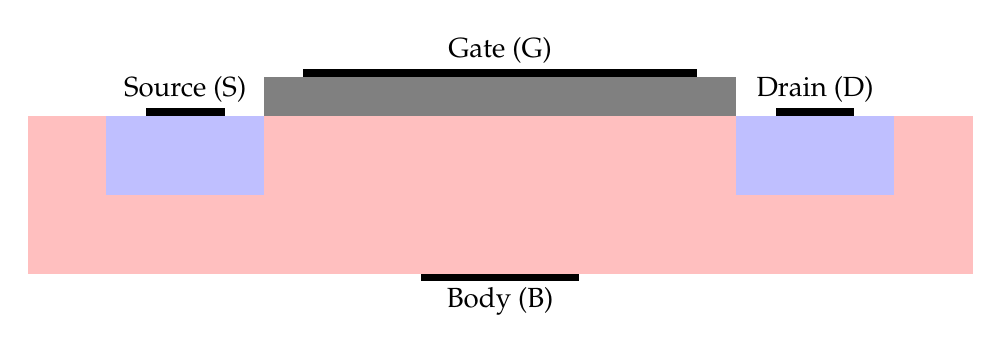
\begin{tikzpicture}
 	\fill[color=red!25]  (0,0)  rectangle (12, 2) {};
 	\fill[color=blue!25] (1,2)  rectangle (3, 1) {};
 	\fill[color=blue!25] (9,1) rectangle (11, 2) {};
 	\fill[gray] (3,2) rectangle (9,2.5) {};
 	\fill[color=black]  (1.5,2) rectangle (2.5, 2.1)  node[above,pos=0.5]{Source (S)} {};
 	\fill[color=black]  (9.5,2) rectangle (10.5, 2.1) node[above, pos=0.5]{Drain (D)} {};
 	\fill[color=black] (3.5, 2.5) rectangle (8.5, 2.6) node[above, pos=0.5]{Gate (G)} {};
 	\fill[color=black] (5, 0) rectangle (7, -0.1) node[below,pos=0.5]{Body (B)};
 \end{tikzpicture}
 \end{center}

 \subsection{Structure}

 Where blue is P-type silicon, red is N-type (often you will see $n^+$ to denote that it is `heavily' doped, and $n^-$ would be lightly doped), black is metal, and gray is SiO$_2$ (the oxide part of NMOS). The thickness of this oxide layer is important, and denoted $t_{\text{ox}}$. The body is typically connected to the \textbf{source}. The Source and Drain are interchangable - there is no intrinsic difference between them in the structure of the NMOS, so the drain is whichever terminal is more positive in a given circuit - current \textbf{always} flows from drain to source.

 \subsection{Operation}
 Applying a positive voltage at the gate (relative to the source) causes an electric field that pushes holes in the substrate down towards the body terminal. When the applied voltage $V_{\text{GS}}$ exceeds $V_t$, a \textbf{channel} is established - the p-type substrate essentially flips to n-type and allows electrons to flow. It is useful to define the \textbf{overdrive voltage}

 \begin{equation}
 	\label{eqn:overdrive-voltage}
 	V_\text{OV} = V_\text{GS} - V_t
 \end{equation}

When $V_\text{DS}$ is small, we can compute the charge in the channel as

\begin{align}
	\label{eqn:nmos-channel-charge}
	|Q| &= C_{\text{ox}} \cdot W L \cdot V_{\text{OV}} \\
	C_\text{ox} &= \frac{\epsilon_\text{ox}}{t_\text{ox}}
\end{align}

 There are three regions of operation, which determine what the current $I_{\text{DS}}$ is. Note first the following definitions:

 \begin{align}
 	\label{eqn:transconductance}
 	k_n' &= \mu_nC_\text{ox} \\
 	k_n &= \left(\frac{W}{L}\right)k_n'
 \end{align}

$k_n'$ is called the \textbf{process transconductance} parameter.

 \begin{align}
 	\label{eqn:nmos-regions-of-operation}
 	\text{Triode} \ \ \ \ i_{DS} &= k_n\left(V_{OV} - \frac{1}{2}v_{DS}\right)v_{DS}\\
 	\text{Saturation} \ \ \ \ i_{DS} &= \frac{1}{2}k_nV_{OV}^2\\
 	\text{Cut-Off} \ \ \ i_{DS} &= 0
 \end{align}

 When $V_{OV} < 0$, the NMOS is in cutoff. When $V_{OV} \ge 0$, there are two cases:

 \begin{itemize}
 	\item $v_{DS} < V_{OV}$: Triode
 	\item $v_{DS} \ge V_{OV}$: Saturation
 \end{itemize}

Note that in triode, with small $v_{DS}$, the $v_{DS}^2$ term can be omitted and thus the transistor acts as a linear resistance between the source and drain controlled by $V_{OV}$:

\begin{equation}
	\label{eqn:linear-resistance-nmos}
	r_{DS} = \frac{1}{k_nV_{OV}}
\end{equation}

\section{PMOS}
PMOS is the opposite of NMOS, and all the equations work out the same if you use the parameters $V_{SG}, V_{SD}$, and $|V_{tp}|$. In PMOS, applying a \textbf{negative} voltage at the gate establishes a channel. The drain is always the more \textbf{negative} of the two terminals, and current always flows from \text{source to drain} (these two statements are the opposite as those for the NMOS).

\section{MOSFET Circuits}
To solve DC MOSFET circuits, you will sometimes need to \textit{assume} regions of operation for each transistor, solve the currents/voltages, and then confirm that the assumptions were correct.

\section{Secondary Effects}

\subsection{Channel-Length Modulation}
In saturation, using the \textbf{long-channel} model we have assumed, the transistor has infinite output resistance. This is not true as in reality, increasing $v_{DS}$ causes channel length modulation. That is, it shortens the channel and increases the potential drop between the channel and the other terminal, slightly increasing the current. This is modelled by adding the factor $\lambda = \frac{1}{V_A}$ to the saturation current where $V_A$ is the `Early voltage', as seen in \ref{eqn:clm-sat-current}. This results in a \textbf{finite} output resistance $r_o$ given by \ref{eqn:clm-sat-resistance}

\begin{equation}
	\label{eqn:clm-sat-current}
	i_{DS} = \frac{1}{2}k_nV_{OV}^2 (1 + \lambda V_{DS})
\end{equation}

\begin{equation}
	\label{eqn:clm-sat-resistance}
	r_o = \frac{1}{\lambda I_{D}}
\end{equation}


\chapter{CMOS Logic}

\section{CMOS Gates}

\subsection{Switches}
It is pure \textbf{convention} that a logical 1 is considered to be a high voltage, e.g. $V_{DD}$ and a logical 0 is GND. Regardless, with this convention in mind, we can treat a NMOS transistor as a switch that is ON when provided with a logical 1 and OFF otherwise. Similarly, a PMOS is a switch that is ON when provided with a logical 0 and OFF when provided with a logical 1. By `provided' we mean the logical value is presented at the gate, and the switch is ON when it connects the drain terminal to the source.

\subsection{Static CMOS Inverter}

\begin{figure}
	\centering
	\begin{circuitikz}
		\draw (-0.5,0) node[left]{X} -- (0,0);
		\path (1.5, 1.5) 	node(P)[pmos]{};
		\path (1.5, -1.5) 	node(N)[nmos]{};
		\path (1.5, 2) 		node(VDD)[vcc]{};
		\path (1.5, -2) 	node(GND)[ground]{};
		\draw (0,0) |- (P.G);
		\draw (0,0) |- (N.G);
		\draw (P.D) -- (N.D);
		\draw (P.S) -- (VDD);
		\draw (N.S) -- (GND);
		\draw (P.D) ++(0,-.75) -- ++(1,0) node[right]{Y};
	\end{circuitikz}
	\caption{A Static CMOS Inverter}\label{fig:static-cmos-inv}
\end{figure}

\autoref{fig:static-cmos-inv} shows the circuit. Some notable features:
\begin{itemize}
	\item Exactly one path (through Q1 or Q2) is active for any input, so there is no middle state output
	\item Input is connected to the gates of MOSFETs, so there is low input leakage
	\item The input is electrically isolated from the output
\end{itemize}

\subsection{Static CMOS Logic}
In general, a static CMOS gate has the structure shown in \autoref{fig:static-cmos}. The pull-up network (PUN) is formed with PMOS, while the pull-down network (PDN) is formed with NMOS. To find the PDN for a function $y = f(\vec{x})$, apply DeMorgan's rules (\ref{eqn:demorgan-1} and \ref{eqn:demorgan-2}) to find $\bar{y}$ as a function of the inputs, and use transistors in series to implement AND and transistors in parallel to implement OR. Then complement the PDN to find the PUN (using parallel PMOS in the PUN to correspond to series NMOS in the PDN and so forth).

\begin{figure}[h]
\centering
\begin{circuitikz}
	\draw (0,3) rectangle (2, 5) node[pos=0.5]{PUN};
	\draw [->] (1,5) to (1, 6);
	\draw (0,0) rectangle  (2, 2) node[pos=0.5]{PDN};
	\draw [-] (1, 2) -- (1, 3);
	\draw [-] (1, 2.5) -- (2, 2.5) node[pos=1.5]{out};
	\draw [-] (1, 0) to (1, -1) node[ground]{};
	\draw [-] (-2, 2.5) -- (-1, 2.5) node[pos=-0.5]{in};
	\draw [-] (-1, 1) -- (-1, 4);
	\draw [-] (-1,4) -- (0, 4);
	\draw [-] (-1, 1) -- (0, 1);
\end{circuitikz}
\caption{Structure of a static CMOS gate}\label{fig:static-cmos}
\end{figure}



\begin{equation}
	\label{eqn:demorgan-1}
	\overline{(A + B)} = \overline{A} \ \overline{B}
\end{equation}
\begin{equation}
	\label{eqn:demorgan-2}
	\overline{AB} = \overline{A} + \overline{B}
\end{equation}

\section{Inverter Voltage Transfer Curve (VTC)}

\subsection{Overview}
For the inverter circuit in \autoref{fig:static-cmos-inv}, we can find $V_{out}$ as a function of $V_{in}$ under the \textbf{quasi-static} assumption (rather than \textbf{dynamic}). In this analysis, we assume $V_{in}$ is stable for a long time and that $I_{DN} = I_{DP}$ (the current flowing into the NMOS drain and out of the PMOS drain are equal). There are 5 regions of operation. We can derive the transistor voltages using $V_{in}$ and $V_{out}$ as follows:

\begin{align*}
	v_{DSN} &= V_o \\
	v_{GSN} &= V_i \\
	v_{SDP} &= V_{DD} - V_o \\
	v_{SGP} &= V_{DD} - V_i
\end{align*}

\subsection{Regions of Operation}
A common case for analysis is when the transistors are \textbf{balanced}, that is $k_n = k_p$ and $V_{tn}= |V_{tp}| = V_t$. The regions of operation are as follows, in order of increasing $V_{i}=V_{in}$:


\begin{enumerate}
	\item Region 1 - $V_{in} < V_{tn}$
	\begin{itemize}
		\item By definition, the NMOS is off. $v_{SGP}$ is very high and $v_{SDP}$ is low, so PMOS is in triode
		\item $I=0$ and $V_o=V_{DD}$
	\end{itemize}
	\item Region 2 - $V_{in} \ge V_{tn}$
	\begin{itemize}
		\item NMOS turns ON, and PMOS is still in triode
		\item NMOS will be in saturation as $v_{DSN}$ is large
		\item Output begins to discharge through the NMOS, but PMOS remains triode until $v_{SDP} \ge v_{SGP} - |V_{tp}|$, which is equivalent to $V_o \le V_i + |V_{tp}|$
		\item So region 2 ends when $V_o$ decreases to $V_i + V_{tp}$
		\item By the quasi-static condition, we have $\frac{1}{2}k_n(v_{GSN} - V_{tn})^2 = k_p(v_{SGP} - |V_{tp}| - \frac{1}{2}v_{SDP})v_{SDP}$, from which we can find $V_o$ as a function of $V_i$ in this region.
	\end{itemize}
	\item Region 3 - $V_i = V_M$
	\begin{itemize}
		\item Both PMOS and NMOS in saturation
		\item $V_M - V_{tn} \le V_o \le V_i + |V_{tp}|$
		\item When \textbf{balanced}, $V_M = \frac{1}{2}V_{DD}$ and $V_{tn}=|V_{tp}|=V_t$ so $|V_0 - \frac{1}{2}V_{DD}| \le V_t$
		\item If we let $r = \sqrt{\frac{k_p}{k_n}}$, we can analyze how $V_M$ shifts: $r > 1$ means \textbf{PMOS} is stronger, so $V_M$ shifts to the right. Intuitively, the minimum $V_{SGP}$ required to turn the PMOS on is now lower, so that region shifts right.
	\end{itemize}
	\item Region 4 - $V_{in} \le V_{DD} - |V_{tp}|$
	\begin{itemize}
		\item NMOS in triode, PMOS turns ON in saturation
		\item Mirrors region 2
	\end{itemize}
	\item Region 5 - $V_{in} \le V_{DD}$
	\begin{itemize}
		\item NMOS in triode, PMOS is cut off
		\item Mirrors region 1
	\end{itemize}
\end{enumerate}

Note that these assume that there is no channel length modulation. Adding the CLM factor will give a finite width for region 3 that has a slight slope.

If we were to do something similar for the drain current as a function of input voltage, we would find a curve that is 0 when the input is near a logic 0 or 1, and a spike at around $V_M$ ($\frac{V_{DD}}{2}$ for balanced circuit). This is related to the dynamic or `switching' power - it takes energy to switch this circuit.

\subsection{Noise Margins}
Noise margins determine how much noise the circuit can tolerate. There are two noise margins, the margin for low input NM$_L = V_{IL} - V_{OL}$ and the margin for high input NM$_H = V_{OH} - V_{IH}$. The overall noise margin NM is the \textbf{minimum} of the two.

\begin{itemize}
	\item $V_{IL}$ is the maximum input that will be considered a 0
	\item $V_{IH}$ is the minimum input that will be considered a 1
	\item $V_{OL}$ is the maximum output value that will be produced when it should be a 0
	\item $V_{OH}$ is the minimum output value that will be produced when it should be a 1
\end{itemize}

The definition we adopt in this course is that these values are defined by the two points on the inverter VTC where $\frac{\partial V_o}{\partial V_i} = -1$. The lower one is $(V_{IL}, V_{OH})$ and the upper is $(V_{IH}, V_{OL})$.

\chapter{Dynamic CMOS Behaviour}
In this section we look at the response of CMOS circuits in the \textbf{dynamic} situation. We no longer assume the quasi-static case. The main focus here is the \textbf{delay}, although in modern technologies power equally if not more important. We begin with the following definitions (with a static CMOS inverter in mind):

\begin{itemize}
	\item Switching delay $t_{pLH}$ and $t_{pHL}$, which is the time from the switching point of the input to the time when the output becomes high or low respectively
	\item Propagation delay $t_p = \frac{t_{pHL} + t_{pLH}}{2}$
	\item Fall time $t_{f}$ (90\% $V_{DD}$ to 10\%$V_{DD}$)
	\item Rise time $t_{r}$ (10\% $V_{DD}$ to 90\%$V_{DD}$)
\end{itemize}

\section{RC Delay Model}
The full analysis is complex, so we assume a simple linear model where the transistor is a resistor in series with a switch and some capacitance.

\begin{figure}[h]
\centering
\begin{circuitikz}
    \draw (0,0) node[ground]{} to[R=R] (0,2) -- (2,2) to[C=C] (2,0) -- (0,0);
    \draw (0,2) to[normal open switch] (0,4) node[vcc]{$V_{DD}$};
\end{circuitikz}
\caption{RC model of a transistor} \label{fig:NMOS-RC-model}
\end{figure}

In this model, the output response to a step input will be an exponential decay with time constant $\tau$. The capacitance and resistance are functions of the transistor aspect ratios. The NMOS and PMOS of a given technology will have some effective resistance $R$. If we scale the width of a transistor by a factor $k$, we get the following effects:

\begin{align}
	\label{eqn:scaled-R}
	R' &\xleftarrow{} \frac{R}{k}\\
	\label{eqn:scaled-C}
	C' &\xleftarrow{} kC
\end{align}

That is, the capacitance goes up and the resistance goes down (in turn increasing the current the transistor can supply).

\section{Sizing a Single Stage}\label{sec:sizing-single-stage}
The goal in sizing one stage of a circuit is to get $t_{pHL} = t_{pLH}$. This is accomplished by computing the 'effective widths' of the PUN and PDN in \autoref{fig:static-cmos}. The effective width of the PUN should equal the width of the PMOS in the technology's basic inverter (called the \textbf{unit inverter}). The effective width of the PDN should equal the width of the NMOS in the basic inverter.

Given $\mu_p$ and $\mu_n$, the first step is to find the relative sizes in the basic inverter. Since $k = \mu C_{ox} \frac{W}{L}$ and $L$ and $C_{ox}$ are typically fixed values, $k \propto \mu W$ and thus we have $\mu_NW_N = \mu_pW_P$ to balance the inverter. Thus we have the ratio $\frac{W_P}{W_N} = \frac{\mu_N}{\mu_P}$. Given a value of $W_N$ we can solve for $W_P$.

The goal is to get the PUN to sum up to $W_P$ and the PDN to sum up to $W_N$ by assigning the width of each transistor to be some multiple of $W_P$ and $W_N$ respectively. In series, the effective width will be given by \autoref{eqn:sizing-width-series} and in parallel they simply add up. So for example, if we have N transistors in series they should all be N times the unit width to get the correct sum. \textbf{Important} in the parallel case, we need \textit{each branch} to be equal to the basic width since a single branch supplying current is the `worst case' for supplying current, and we want the worst case delays to be equivalent to the unit inverter.

\begin{equation}
	\label{eqn:sizing-width-series}
	\frac{1}{W_e} = \frac{1}{W_1} + \frac{1}{W_2}
\end{equation}

\section{Elmore Delay} \label{sec:elmore-delay}
A more useful RC model for the delay is given by \autoref{fig:NMOS-Detailed-RC}. Note that the resistances and capacitances are determined by \autoref{eqn:scaled-R} and \autoref{eqn:scaled-C}.

\begin{figure}
\centering
\begin{circuitikz}
	\draw (0,0) -- ++(1,0) to[C=C] +(0,-1) node[ground]{};
	\draw ++(3,0) to[normal open switch] ++(0,2) node[above]{D} to[R=R] ++(2,0) to[C=C] +(2,0) node[ground]{};
	\draw ++(3,0) -- ++(0,-2) node[below]{S} -- ++(2,0) to[C=C] ++(2,0) node[ground]{};
\end{circuitikz}
\caption{NMOS RC Model}\label{fig:NMOS-Detailed-RC}
\end{figure}


Using this, and noting that the capacitances connected to a constant supply may as well be connected to ground, we can draw out the full RC model for the inverter, shown in \autoref{fig:Inverter-RC}. Note that technically there are 3 process-dependent capacitances $C_g, C_s, C_d$ (and technically even more), but this is a \textit{first-order} assumption that they are all equal to $kC$ where $C$ is the unit width capacitance.

Also note that \autoref{fig:Inverter-RC} assumes the PMOS was scaled by 2, which decreased its effective resistance to be the same as that of the NMOS path.

Delay calculations are based on the \textbf{Elmore delay}. Simply put, we estimate the delay of a path in an RC network by taking the sum of the delay at each R along the path. The delay at a node with a resistance R is $RC_p$ where $C_p$ is the sum of the capacitances from the node R to the desired output node. For example, the delay in the network of \autoref{fig:elmore-example} is $R(C + 2C) + \frac{R}{4} (2C)$.

\begin{figure}
\centering
\begin{circuitikz}
	\draw node[ground]{} (0,0) to[R=R] (0,2)	-- (1,2) to[C=C] (1,0) node[ground]{};
	\draw (1,2) -- (3,2) to[R=$\frac{R}{4}$] (3,0) node[ground]{};
	\draw (3,2) to (5,2) to[C=$2C$] (5,0) node[ground]{};
\end{circuitikz}
\caption{Simple Elmore delay example}\label{fig:elmore-example}
\end{figure}



\begin{figure}
\centering
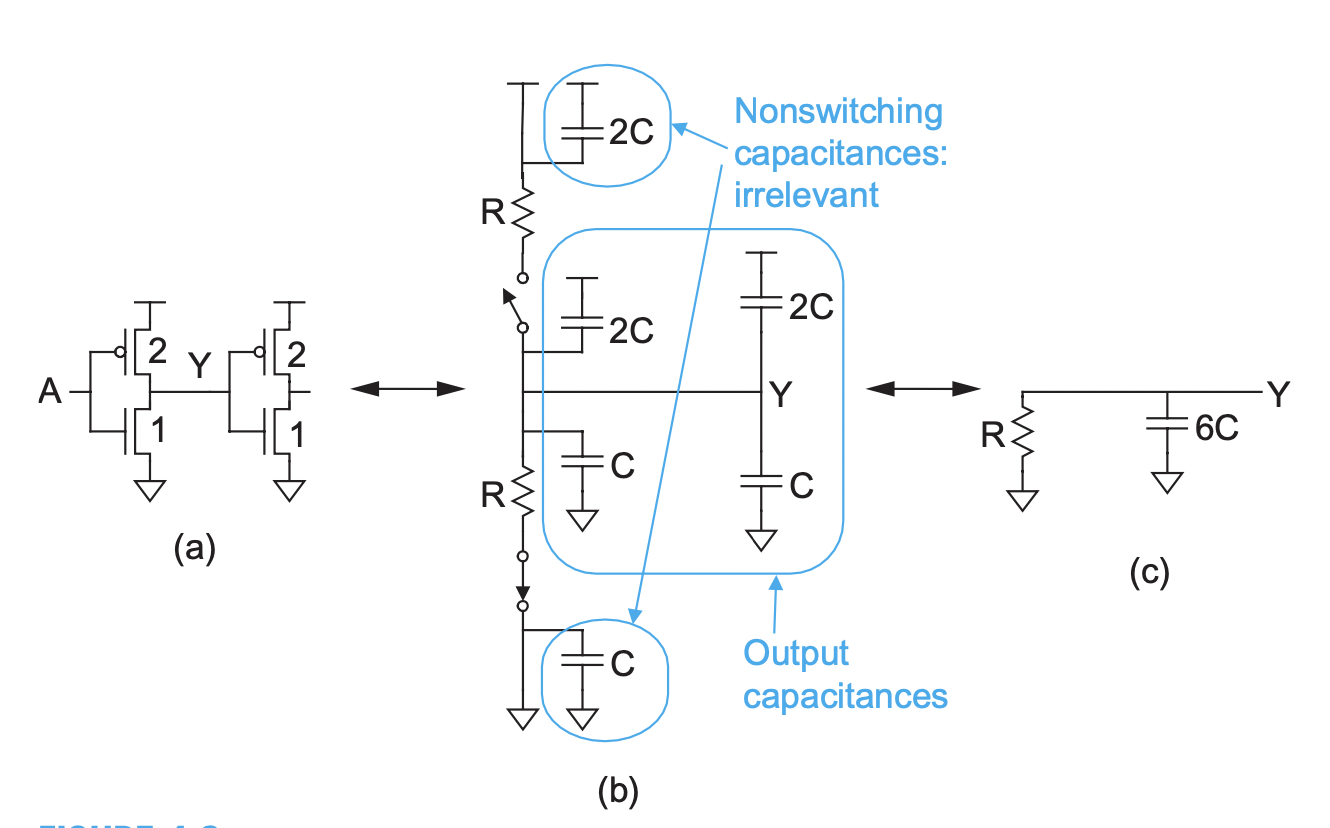
\includegraphics[scale=0.5]{images/cmos-inv-RC.png}
\caption{The full RC model of the inverter}\label{fig:Inverter-RC}
\end{figure}

\section{Power}

\subsection{Dynamic Power}
Charging a capacitor to some voltage takes energy. The power is given by $P(t) = I(t)V(t)$ and the energy is $E = \int_{0}^{\infty}P(t)dt$. When a source at voltage $V_{DD}$ charges the capacitor to $V_{DD}$, it delivers a current $i_c(t) = C\frac{dv_c(t)}{dt}$ and thus uses energy

\begin{equation}
	E_{supply} = \int_{0}^{\infty} C\frac{dv_c(t)}{dt}V_{DD}dt = CV_{DD}\int_{0}^{V_{DD}}dv_c = CV_{DD}^2
\end{equation}

Meanwhile, the energy stored in the capacitor is given by

\begin{equation}
	E_C = \int_0^\infty C\frac{dv_c(t)}{dt}v_c(t)dt = C\int_0^{V_{DD}} v_c(t) dv_c = \frac{1}{2}CV_{DD}^2
\end{equation}


That is, half of the energy given by the supply is stored on the capacitor and the other half is dissipated. In a CMOS inverter, we thus have that every time the \textit{output} has to go from 0 to 1, it dissipates $\frac{1}{2}CV_{DD}^2$ Joules of energy. When the output then has to go from 1 to 0, the capacitor discharges through the NMOS (\textbf{the supply does not provide any energy}) and dissipates $\frac{1}{2}CV_{DD}^2$.

Note that the average power in a period $T$ is given by $P_{av} = \frac{E}{T}$ where $E$ is the energy used in that period. Consider the clock. In one period, it must make \textbf{both} transitions (1 to 0 and 0 to 1), thus the average power of a clock with period $T$ is $\frac{1}{T}(\frac{1}{2}CV_{DD}^2 + \frac{1}{2}CV_{DD}^2) = \frac{1}{T}CV_{DD}^2 = fCV_{DD}^2$ where $f$ is the clock frequency. Similarly, for a signal that switches on average $\alpha$ fraction of the time, the power is

\begin{equation}
	\label{eqn:dyn-power-alpha}
	P_{dyn} = \alpha f CV_{DD}^2
\end{equation}

Where $\alpha$ is the activity factor. Note that the activity factor for the clock is \textbf{always} 1. For a signal that switches value, the activity factor is 0.5 (\textbf{very important} - it is \textit{not} 1 because such a signal actually only changes value half as often as the clock).

If you are given a signal over $N$ clock periods, you can find the activity factor by counting $k$, the number of edges depicted, and the activity factor is $\frac{k}{2N}$

An alternative definition of $\alpha$ is the probability that a signal switches from a 0 to a 1.

\subsection{Subthreshold Leakage}\label{sec:subthreshold}

In modern technologies, we actually have a nonzero drain current even when $v_{gs} < V_t$ (similar for PMOS). This is proportional to a few things, and the current is usually given in a datasheet. In general,

\begin{equation}
	\label{eqn:subthreshold-current}
	I_D = I_0 e^{\frac{v_{gs}}{\frac{nkT}{q}}}	\left(1 - e^{-\frac{v_{ds}}{\frac{kT}{q}}}\right)
\end{equation}


\subsection{Static Power Dissipation}
Due to subthreshold leakage (\autoref{sec:subthreshold}), the NMOS and PMOS of a gate will leak power even when they are not switching. Given base values for the currents, $I_{N0}$ and $I_{P0}$, we can compute an estimate for the static power by multiplying them by the widths of the sized transistors.

To estimate the power, we need to consider two cases. When the output is a 1 ($V_{DD}$), only the leakage current of the \textbf{NMOS} consumes power. This is because $v_{sdp} = 0$ and thus the current $I_{D}$ is 0 in \autoref{eqn:subthreshold-current}. When the output is a 0, only the leakage current of the \textbf{PMOS} consumes power, for similar reasons.


Thus, for a given set of inputs, you can estimate the static power as follows. Find the output, and determine whether the NMOS or PMOS case is to be considered. Then find the effective width of the transistors that are OFF, and the power is $w_eI_0V_{DD}$ where $w_e$ is the effective width and $I_0$ is the per-width leakage current for that type of transistor (NMOS or PMOS).


\chapter{Combinational Circuits}
\section{The Logic Effort Method}

\subsection{Single Stage}
We need some way of intuiting which design for a given boolean function is good. The delay is what we focus on here, though power is also important. So, for a given topology, how can we quickly estimate the delay? Using the Elmore delay of \autoref{sec:elmore-delay}. We would like to see how a single logic gate performs in a given circuit. The delay of a gate that is connected to some other gates is given by the product $R(C_{parasitic} + C_{load}) = R(C_{parasitic} + C_{in}\cdot\frac{C_{load}}{C_{in}})$.
\begin{itemize}
\item $R$ is the path resistance which has been designed to be equal to the path resistance of the basic inverter (see \autoref{sec:sizing-single-stage})
\item $C_{parasitic}$ is the capacitance at the output of the logic gate, which depends on what transistors are connected to the output node of the logic gate and what their sizes are\
\begin{itemize}
	\item What makes it parasitic? Well because ideally we would want it to be 0 so we can just drive the load capacitances (which by their very existence are non-zero). It is non-zero because we need to use transistors to do this, which come with some output capacitance.
\end{itemize}
\item $C_{load}$ is the input capacitance of the total load that the logic gate drives (i.e. the sum of input capacitances of all the gates it drives)

\end{itemize}
We can write that delay also in the following manner:

\begin{equation}
\label{eqn:logic-effort-delay}
	d = p + f = p + gh
\end{equation}

Let the delay of the unit inverter be $\tau_0$ (e.g. $\tau_0 = 3RC$ if $\mu_n = 2\mu_p$) and the 'unit capacitance' $C_0$ = $\frac{\tau_0}{R}$. Note the following:

\begin{equation}
	\tau_0 = \left(\frac{\mu_n}{\mu_p} + 1\right)RC
\end{equation}
\begin{equation}
	C_0 = \left(\frac{\mu_n}{\mu_p} + 1\right)C
\end{equation}



\begin{itemize}
\item $d$ is the \textbf{normalized} delay $\frac{\tau}{\tau_0}$ - that is, to get the actual time constant we need to multiply it by $\tau_0$.
\begin{itemize}
	\item Why normalize? Since reducing R or C always decreases delay, and the $\mu_p$:$\mu_n$ ratio changes the unit inverter delay, normalizing it makes sure that all the technology-dependent factors are absorbed into $d$ and we can just worry about relative values
\end{itemize}
\item $p$ is the normalized parasitic delay $\frac{C_{parasitic}}{C_0}$. It is \textbf{independent} of the transistor sizes in the gate.
\item $f = gh$ is the 'stage effort', i.e. the effort that this logic gate has to put in.
\item $g = \frac{C_{in}}{C_0}$ is called the 'logical effort'. It is a measure of the complexity of a gate, and can change with the widths of the transistors (sum of gate capacitances)
\begin{itemize}
 	\item Since this is related to the input capacitance which is proportional to the transistor widths, this is sort of like a measure of how much current this gate can deliver relative to that of the basic inverter
\end{itemize}

\item $h = \frac{C_{load}}{C_{in}}$ is called the 'fan-out' or 'electrical effort' factor. It's the ratio of the load capacitance of the logic gate to its input capacitance (or, if a gate is driving $n$ gates identical to itself, $h=n$ which is where 'fan-out' comes from)
% TODO: better reason?
\begin{itemize}
	\item Why the \textit{ratio} of load to input capacitance and not just the load capacitance? This is just so that the full path-effort method has a nice form ($H$ can be computed as fixed for a given logic block) that can be optimized
\end{itemize}

\end{itemize}

\subsection{Path Logic Effort}
We need one more piece, which is the branching effort for a path $b = \frac{C_{load on path} + C_{load off path}}{C_{load on path}}$. In any circuit there is some critical path whose delay limits the frequency it can be operated on. We introduce three terms that can be computed for the path which has $N$ stages:

\begin{align}
	\text{Path Effort} \ \ \ \ F &= \prod f_i = \prod g_ih_i\\
	\text{Path Logic Effort} \ \ \ \ G &= \prod g_i\\
	\text{Path Branch Effort} \ \ \ \ B &= \prod b_i\\
	\text{Path Electric Effort} \ \ \ \ H &= \frac{C_{out, path}}{C_{in, path}}\\
	\text{Path Parasitic Delay} \ \ \ \ P &= \sum p_i\\
	\text{Path Effort Delay} \ \ \ \ D_F &= \sum g_ih_i\\
	\label{eqn:overall-delay}
	\text{Path Delay} \ \ \ \ D &= P + D_F
\end{align}

Note that $F = GBH$. The goal is to minimize $D$ by selecting $h_i$. That is, we have fixed a circuit topology and want to size each gate (i.e. select the $W_N$ since the ratio of $W_P:W_N$ has already been decided). How do we do it? $P$ is fixed so we want to minimize $D_F$ which can be done by selecting all the $g_ih_i$ terms to be \textbf{equal}. That is, we want to find the optimal \textbf{stage effort} $\hat{f}$:

\begin{equation}
	\hat{f} = g_ih_i = F^{\frac{1}{N}}	\ \ \ \  \ \forall i
\end{equation}

If we do this, the minimum delay is given by

\begin{equation}
	\hat{D} = P + N\hat{f} = P + NF^{\frac{1}{N}}
\end{equation}

The process for a given circuit and path is as follows

\begin{enumerate}
	\item Size each gate (pick widths relative to $W_N$)
	\item Compute $g_i$ and an expression for each $h_i$
	\item Compute $G, B, H,$ and thus $F$. Compute $P$
	\item Compute $\hat{f} = F^{\frac{1}{N}}$. Compute $\hat{D} = P + N\hat{f}$.
	\item Using $\hat{f} = g_ih_i$, compute a value for the input capacitance (this will be for a \textit{single input} of the gate)
	\item Using the input capacitance from the previous stage, write an expression for $W_N$
\end{enumerate}

 For example of step 6, if the input capacitance is $x$ for an input A, and the total input capacitance for the gate is given by $kW_n + jW_p$ and $W_p = \frac{\mu_n}{\mu_p}W_n$, we can write

 $$
 x = kW_n + j\frac{\mu_p}{\mu_n}W_n \implies W_n = \frac{x}{k + j\frac{\mu_p}{\mu_n}}, \ \ \ \ W_p = \frac{\mu_p}{\mu_n}\frac{x}{k + j\frac{\mu_p}{\mu_n}}
 $$

From which we can find the absolute widths $kW_n$ and $jW_p$.

\subsection{Adding Inverters}
It is possible that adding a chain of inverters to the end of a logic block can, by scaling each element of said change, \textit{decrease} the overall delay. If we let $\rho = \hat{f} = F^{\frac{1}{N}}$ and differentiate \autoref{eqn:overall-delay} w.r.t. N, this is given by

\begin{equation}
	p_{inv} + \rho (1 - \ln\rho) = 0
\end{equation}

Since this is not exactly solvable, we use the estimate $\rho \approx 4$ to get

\begin{equation}
	\label{eqn:best-stages}
	N_{best} = \log_4(F)
\end{equation}

Note that $N_{best} = N_{orig} + n_{inv}$.


\section{Other Delay Reduction Methods}
\subsection{Gate Topology: Inner vs. Outer Inputs}\label{sec:inner-outer}
Think of the Elmore delay of an input closer to the rail in a series of transistors connected to some output node. The outer nodes need to charge both the output capacitance and the series capacitance of all the drains/sources of the other transistors.

An \textbf{inner} node is one closer to the output, an \textbf{outer} node is closer to the rail. If we know which inputs arrive later than others, we should always put the latest input at the \textit{innermost} node, so it has to charge the least capacitance.


\subsection{Layout: Shared Capacitance}
For transistors in series, using the n-well of one transistor's drain as the n-well for another transistor's source, can reduce the output node capacitance from $2C + 2C$ to just $2C$

\subsection{Layout: Multi-Finger Devices}
For very wide transistors, we can use N fingers to lay it out instead. N is the number of places the gate touches the device. This reduces the source/drain capacitances while maintaining the channel width.

\subsection{Transistor Sizing: Asymmetric Gates}
When we know one input is more critical than another, for example a reset, we can reduce its delay by reducing the widths of the transistors it is connected to. We must proportionally \textit{increase} the widths of the other transistors to maintain the single-stage sizing.

\subsection{Transistor Sizing: Skewed Gates}
If a rising output of an inverter is more critical, we can downsize the nMOS so that the charging resistance is now proportionally larger than the discharging resistance.


\section{Alternative Logic Families}
Static CMOS is just one way to implement boolean functions.

\subsection{Pseudo-NMOS}
PMOS is slow, so what if we could omit it entirely? In pseudo-NMOS we use a very weak PMOS with its gate connected to ground (always-on) that serves as a pull-up resistor (why not just use a resistor? It would use more space in a CMOS technology). Then we implement our PDN as usual using NMOS.

When the output should be a 1, the PDN is disconnected and the output charges through the PMOS. When it should be a 0, the PDN pulls it down (and fights with the PMOS pullup!). This means that there is a lot of static power usage when the output should be a 0 (not when it should be a 1 as no current flows across the resistor).

Pseudo-NMOS has fast $1\xrightarrow{}0$ transitions but slow $0 \xrightarrow{}1$ transitions. It has lower noise margins than static CMOS, and uses more power.


\subsection{Pass-Transistor Logic}\label{sec:pass-transistor-logic}
This logic family only uses NMOS gates. The idea is to use both the gates and source/drains of the transistors as inputs.

\subsubsection{Pass-Gate}
A 2-input PTL gate is implemented as follows. For inputs A,B there are two NMOS transistors Q1 and Q2. Q1 has its gate connected to B and Q2 has its gate connected to $\bar{B}$. The source of Q1 and the source of Q2 are each connected to one of $\{A, \bar{A}, 0, 1\}$. The drains of Q1 and Q2 are connected.

Unlike static CMOS, we must \textbf{ensure} that exactly one path is conducting (Q1 or Q2). We can implement $2^4$ functions in this family. This family is good for reducing the number of transistors in specialized applications like FPGA matrices and memories.

\subsubsection{$V_{th}$ Drop}
When G=1 and D rises to 1 in an NMOS transistor, S will rise (since it is a resistor with G fixed) until $V_S = V_{DD} - V_t$ at which point $V_{GS} = V_{DD} - (V_{DD} - V_t) = V_t$ and the transistor becomes cut-off. Therefore the 'output' in this logic family for a $V_{DD}$ is $V_{DD} - V_t$. This is called the \textbf{$V_{th}$ drop} and means that \textbf{the output of a PTL gate cannot be used as the gate input to another PTL gate}. It can be used as the drain input, provided $V_{DD}-V_{t}$ is large enough, but using it as the input to a gate means the next output will be $V_{DD} - 2V_{t}$ and so on.

\subsubsection{Transmission Gates}
A transmission gate is a NMOS-PMOS pair with the source of one connected to the drain of the other and vice versa. The input is a value $X$ where $X$ is passed to the gate of one transistor and $\bar{X}$ is connected to the gate of the other.

This essentially implements a \textbf{switch} that doesn't have a $V_{th}$ drop. If $X$ is connected to the NMOS, the switch turns on when $X=1$. If $\bar{X}$ is connected to the NMOS instead, the switch turns on when $X=0$.

\subsubsection{Complementary Pass-Transistor Logic (CPL)}
If we use pass-gate logic to implement both $F(A,B)$ and $\bar{F}(A,B)$, we can assume that all inputs to a logic gate have both polarities provided, and using a CMOS inverter to restore the logic levels we can reduce the number of inverters required.

\subsection{Dynamic Logic}
In dynamic logic, we rely on some node's capacitance to store a voltage rather than directly connecting it to some pull-up or pull-down.

General characteristics of `dynamic' things:
\begin{itemize}
	\item They use the capacitance of some node to store charge
	\item Higher density
	\item Less robust
	\item Higher power
	\item Fast
\end{itemize}

Dynamic logic has the drawback that the clock needs to be slow enough for precharging.

\subsubsection{Clocked-Evaluation Dynamic Logic}

\autoref{fig:clocked-eval-dynamic-gate} shows the schema. In the \textbf{precharge} phase, the clock is low and the output node is charged to a 1. In the \textbf{evaluation} phase the clock is high and the output is equal to the function implemented by the PDN. There is one important exception: once Y discharges through the PDN, it cannot rise as the PMOS is disconnected. This is called \textbf{monotonicity}, and means that the output of such a logic gate cannot cascade to other similar logic gates unless monotonicity is guaranteed.

Note that the NMOS at the bottom of \autoref{fig:clocked-eval-dynamic-gate} is called a \textbf{foot} - if we can guarantee the inputs are never $1$ during evaluation, we can omit the foot and reduce the load capacitance of the clock.

We can decrease the logical effort for inputs in the PDN by \textit{increasing} the width of the foot. The drawback is that this increases the clock load.

The pull-up transistor is usually given $\frac{1}{2}R$ so the precharge occurs quickly.

If we had some way of guaranteeing that no input goes from $1 \xrightarrow{} 0$, then everything would be okay. This is what leads us to \textbf{domino} logic.

\begin{figure}[h]
\centering
\begin{circuitikz}
\draw (0,1)rectangle(2,2)
(1,2) -- (1, 3){}
to [short,*-o] ++(1,0) {} node[right=2mm] {Y}
(1,4) node[pmos](pmosB){}node[left=10mm] {$\phi$}
(1,0) node[nmos](nmosC){}node[left=10mm] {$\phi$}
(1,5) node[vcc](vcc){}
(1,1) node[above=5]{PDN}
(1,-1) node[ground](gnd){}
(1,1) to (nmosC.D)
(1,3) to (pmosB.D)
(vcc) to (pmosB.S)
(gnd) to (nmosC.S);
\end{circuitikz}
	\caption{Clocked Evaluation Dynamic Logic Gate}\label{fig:clocked-eval-dynamic-gate}
\end{figure}

\subsubsection{Domino Logic}
The term 'monotonically rising' means \textbf{only} that a signal \textit{cannot} go from $1\xrightarrow{}0$. Similarly, a 'monotonically falling' signal may not go from $0 \xrightarrow{} 1$.

If a signal is monotonically falling, then feeding that signal to a static CMOS inverter causes an output that is monotonically rising. This is the idea behind domino logic. We stick some inverting static CMOS gate at the output of a dynamic logic gate and can thus cascade such \textbf{compound gates}. The drawback is that only \textit{noninverting} logic can be implemented (e.g. no NANDs or XORs).

\subsubsection{Zipper Logic}
Consider an altered version of \autoref{fig:clocked-eval-dynamic-gate} where we implement a PUN and feed $\bar{\phi}$ to the transistors instead. Such a gate would have a 'predischarge' phase when $\phi=0$ and in eval allows a monotonically rising \textit{output}. That is, it can \textbf{tolerate monotonically falling inputs}. Thus if we alternate stages of 'positive dynamic logic' (\autoref{fig:clocked-eval-dynamic-gate}) with the described 'negative dynamic logic', we have no issues with monotonicity.

Problems with Zipper logic:
\begin{itemize}
	\item Requires $\phi$ and $\bar{\phi}$ everywhere, which is not an easy task
	\item Greatly increases the activity factor $\alpha$ (usually in the 30\%-40\% range compared to the $\sim1\%$ of static CMOS)
	\item Lower noise margin
\end{itemize}

\subsection{Dynamic Logic Issues}

\subsubsection{Charge Leakage}
Dynamic logic relies on a node's capacitance to store a logic level. In modern processes, due to high leakage, such nodes may only hold their charge on the order of nanoseconds. To solve this we can add a 'weak keeper' which is essentially a level restorer at the output.

\autoref{fig:level-restorer} shows a level restorer. It maintains the node $Y$ at whatever its value is even as it drifts. Suppose $Y$ is a 1 and it begins to discharge to some voltage below $V_{DD}$. As long as this is below the noise margin of the inverter, the inverter will continue to output $\bar{Y}=0$. The $V_{SG}$ of Q1 is held at $V_{DD}$ so it is ON. decreasing $Y$ \textit{increases} $V_{SD}$, increasing the current drawn through Q1 which in turn decreases $V_{SD}$ (thus brining $Y$ back to a 1). A similar analysis holds for keeping a 0. \textbf{Note} that Q1 must be \textbf{weak} enough to be 'overridden' by the logic gate driving $Y$.

\begin{figure}[h]
\centering
\begin{circuitikz}
	\draw
	(0,0) node(keeper)[pmos,rotate=180]{}
		  node(keeper_name)[left]{Q1}
	(0,1) node(vdd)[vcc]{}
	(keeper.S) -- ++(0,-0.5) -- +(0.2,0) node(inv)[american not port, anchor=in]{}
	(inv.out) |- (keeper.G)
	(vdd) to (keeper.D)
	;

	\draw
	(inv.in) -- ++(-1,0) node[pos=1.5]{$Y$}
	(inv.out) -- ++(1,0) node[pos=1.5]{$\bar{Y}$};
\end{circuitikz}
\caption{A CMOS level restorer}\label{fig:level-restorer}
\end{figure}

\subsubsection{Charge Sharing}
The output node of a dynamic circuit has to share charge with the internal capacitances of the logic gate when the PDN is in the ON state. To avoid this, we must also precharge all the internal capacitances, by adding more $\phi$-connected PMOSes to pull them up.

This can also be solved by adding a large load capacitance that can store voltages for long enough.

\section{Process, Voltage, and Temperature (PVT) Variation}
A lot of things can go wrong and we must tolerate some variation in device parameters to improve yield. The three main ones to consider are:

\begin{itemize}
	\item \textbf{Process}: from the actual construction of the device
	\item \textbf{Voltage}: error in the supply voltage
	\item \textbf{Temperature}: due to operating conditions or heat disippation
\end{itemize}


\subsection{Process}
The actual construction of the transistors is an enormously complex process and there are a lot of factors to consider. To the first order, these essentially change the channel length and threshold voltages of PMOS and NMOS. We usually address this by simulating \textbf{process corners} about the relative strengths of the two polarities as seen in \autoref{fig:process-corners}. The lower $V_t$ or $L$ is of a transistor, the faster it is relative to the other.

The middle point is the Typical-Typical case, whereas the other 4 are the corners (Slow-Slow, Fast-Slow, etc.). The information about these corners comes from the foundry who actually makes the chips, and they will say something like '99\% of all chips will be greater than [some specification of the SS corner]'.

Chips that end up being in the FF corner can be 'binned' as more expensive and rated for higher frequency, and the SS ones can be sold for cheaper (though they should still be functional)

\begin{figure}[t]
\centering
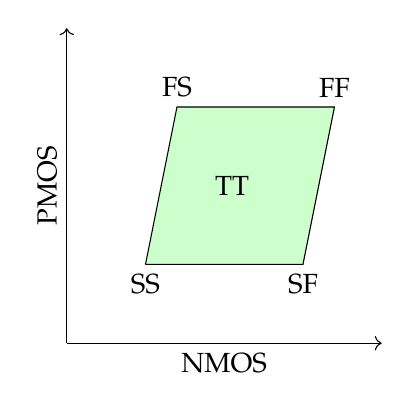
\begin{tikzpicture}
	\draw[->] (0,0) -- (0,4);
	\draw[->] (0,0) -- (4,0);
	\fill[green!20,draw=black]
		(1,1) 		node[below,black]{SS}--
		++(0.4, 2) 	node[above,black]{FS}--
		++(2,0) 	node[above,black]{FF}--
		++(-0.4,-2) node[below,black]{SF}-- (1,1);
	\path(2.1,2) node{TT};
	\path(0,2) node[above,rotate=90]{PMOS}
		 (2,0) node[below]{NMOS};
\end{tikzpicture}
\caption{Process Corner Diagram, Axes in Increasing Speed}\label{fig:process-corners}
\end{figure}

\subsection{Voltage}
Due to various interconnect or supply issues, $V_{DD}$ can typically vary by about $\pm 10\%$. When it is \textit{above} nominal voltage, the chip will be faster but higher power. The opposite is true when it is \textit{below} nominal voltage

\subsection{Temperature}
Note the following relationships

\begin{align}
	Speed &\propto Current\\
		  &\propto Mobility\\
		  &\propto \frac{1}{Bandgap}\\
		  &\propto \frac{1}{T}
\end{align}

Thus as the temperature decreases, we expect the circuit to operate \textit{faster}.


\chapter{Sequential Logic}\label{sec:sequential-logic}
% TODO: FSM and Pipeline diagram
In combinational logic we designed circuits that implement some boolean function over a set of inputs. For a given set of inputs, the output is always the same. In \textbf{sequential logic} we product outputs dependent on the current inputs and the \textit{previous} outputs or the 'state'. There are two styles of sequential logic: \textbf{Finite State-Machine} and \textbf{Pipeline}.

A sequencing element is some circuit that forwards tokens from its input to the output at a regular rate, usually controlled by a clock.

In FSM, there is some combinational logic that feeds into a sequencing element, which feeds back its state every clock cycle. In pipeline, we have N stages of combinational logic separated by sequencing elements. There are two fundamental sequencing elements to consider: latches, which are 'level-triggered' devices, and flip-flops which are 'edge-triggered' devices.


\section{Latches and Flip-Flops}\label{sec:latches-ffs}

A \textbf{Latch} is a circuit with two phases: in the \textit{transparent} (or \textit{follow}) state, the output is equal to the input. In the \textit{hold} state, the circuit holds its previous output independent of the input. A \textbf{positive latch} holds when the clock is low and is transparent when the clock is high. A \textbf{negative latch} holds when the clock is \textit{high} and is transparent when it is low.


A \textbf{Flip-Flop} is a circuit which holds its value except for a small period around a clock \textbf{edge}. In a \textbf{positive edge-triggered flip-flop}, the output takes on the value of the input every positive (i.e. rising) edge of the clock signal. In a \textbf{negative edge-triggered flip-flop}, the output takes on the value of the input every negative (i.e. falling) edge of the clock signal.

The following sections show that if we know how to construct a positive latch, we can construct all polarities of latches and flip-flops. We can then look at how to implement the positive latch using CMOS technology and rely on these constructions to do the rest.

\subsection{Construction of a Negative Latch}
Given a positive latch, we can easily construct a negative latch by simply negating the clock signal.

\subsection{Construction of a Positive Flip-Flop}\label{sec:positive-flip-flop}
If we have a way to implement both positive and negative latches, we can implement either polarity of flip flop. To implement a positive FF, we connect the input to a negative latch which feeds into a positive latch. Call these $L_1$ and $L_2$ respectively. Call the input of latch $i$ $D_i$ and its output $Q_i$. Consider a clock edge that arrives as in \autoref{fig:clock-edge-ff}. Before $t_{\phi1}$, the clock is low and:
\begin{enumerate}
	\item The negative latch is transparent so $Q_1 = D_1$
	\item The positive latch is holding its previous value
	\item The effect of 1 and 2 is that the overall circuit \textit{holds} when clock=0
\end{enumerate}

\begin{figure}[t]
\centering
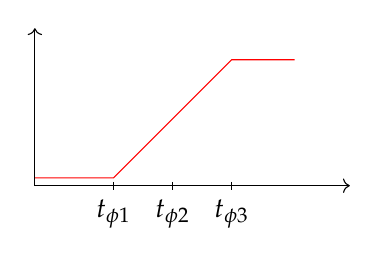
\begin{tikzpicture}
	\draw[red] (0,.1) -- ++(1,0) -- ++(1.5,1.5) -- ++(0.8,0);
	\draw[->] (0,0) -- (0,  2);
	\draw[->] (0,0) -- (4, 0);
	\draw (1,0.05) -- (1,-.05) node[below]{$t_{\phi1}$};
	\draw (1.75,.05) -- +(0,-0.1)node[below]{$t_{\phi2}$};
	\draw (2.5,0.05) --(2.5,-0.05)node[below]{$t_{\phi3}$};
\end{tikzpicture}
\caption{Clock Edge for Flip-Flop Construction}\label{fig:clock-edge-ff}

\end{figure}

When the clock edge arrives ($t_{\phi1}$ to $t_{\phi3}$):
\begin{enumerate}
	\item At some point \textit{after} $t_{\phi1}$, $L_1$ stops following and holds $Q_1$
	\item At some point \textit{before} $t_{\phi3}$, $L_2$ begins following and $Q_2 = D_2 = Q_1$
	\item The effect of 1 and 2 is that by $t_{\phi3}$ the output will take on the value that $L_1$ ended up holding.
\end{enumerate}

Thus we have implemented a positive flip flop that, provided inputs are stable prior to the clock edge, will register and hold the value provided.

\subsection{Construction of a Negative Flip-Flop}

The construction is similar to \autoref{sec:positive-flip-flop}, but with the clock signals negated (i.e. a positive latch followed by a negative one).


\section{Latch Design}
As seen in \autoref{sec:latches-ffs}, we need only focus on the implementation of positive latches. \textbf{In this section, the term 'latch' is equivalent to 'positive latch' unless otherwise specified}.

\subsection{Dynamic Latches}

\subsubsection{Pass-Gate Latch}
The simplest possible latch is a pass gate transistor, seen in \autoref{fig:pass-gate-latch}. It is fast, has low clock load, and only needs $\phi$ (not $\bar{\phi}$). One problem is that it has a $V_{th}$ drop (see \autoref{sec:pass-transistor-logic}), and it allows the output to \textbf{backdrive} the input. It also is dynamic and thus has the same pros/cons as most dynamic circuits.


\begin{figure}[h]
\centering
\begin{tikzpicture}
	\draw (0,0) node(D)[left]{D};
	\path (1,0) node(nmos)[nmos,rotate=-90,anchor=S]{};
	\path (nmos.G) node[above]{$\phi$};
	\draw (nmos.D) to[short,-*] ++(1,0) node(Cstart)[]{} to[C] ++(0,-1) node[ground]{};
	\path (Cstart) node[right]{Q};
	\draw (D) to (nmos.S);
\end{tikzpicture}
\caption{Pass-Gate Dynamic Latch}\label{fig:pass-gate-latch}
\end{figure}

\subsubsection{Transmission Gate}
The transmission gate eliminates the $V_{th}$ drop and requires $\bar{\phi}$. It still allows for backdriving: we can add a static inverter at the output to prevent this. This slows it down but does add isolation and level-restoration.

\subsection{Static Latches}\label{sec:static-latch}
A chain of two static CMOS inverters forms a static latch with some interesting properties. It is known as a \textbf{bi-stable} element since it has two stable states. The two states are logic 0 ($v_{i1} = v_{o2} = 0$) and logic 1 ($v_{i1} = v_{o2} = 1$). To find the properties of the circuit, we can overlay the VTC of each inverter on the same $v_{o1}$ vs $v_{o2}$ plot. What we find is a \textbf{butterfly curve} that has 3 solutions (only the 0 and 1 state are stable). In fact, the two states are self-reinforcing since a small perturbation will cause the state to return to the same value.

We still need some way to write values though, and this is acheived by overpowering the feedback mechanism that keeps the inverter pair in a stable state. This is determined by the point on the butterfly curve where $\frac{\partial v_{o1}}{\partial v_{i1}} = \frac{\partial v_{o2}}{\partial v_{i2}} = 1$

The length of the diagonals in the 'wings' in the butterfly curve determines the static noise margins for the bistable points.

\subsubsection{MUX-Based Latches}
We can implement a latch by a MUX whose select is $\phi$. When $\phi$ is low, the MUX selects the first input, and when $\phi$ is high, the MUX selects the second input. By choosing D to be the first input and Q to be the second input, we get a negative latch. Similarly, if we choose D to be the second input and Q to be the first input, we get a positive latch.

\subsubsection{Tri-State Gate}
A tri-state gate is an efficient way to implement a MUX, seen in \autoref{fig:tristate-gate}.

\begin{figure}
\centering
	\begin{circuitikz}
		\path (0, -3) node(AN)[nmos]{};
		\path (0, -1) node(PN)[nmos]{};
		\path (0, 1) node(PP)[pmos]{};
		\path (0, 3) node(AP)[pmos]{};
		\draw (AN.G) -- (-2, -3) to[short, -o] (-2, 4) node[above]{A};
		\draw (AP.G) to[short, -*] (-2, 3);
		\draw (-3, 1) node[left]{$\overline{\text{EN}}$} -- (PP.G);
		\draw (-3, -1) node[left]{EN} -- (PN.G);
		\path (0, -4) node(gnd)[ground]{};
		\path (0, 4) node(vdd)[vcc]{};

		\draw(AN.S) -- (gnd);
		\draw(AN.D) -- (PN.S);
		\draw(PN.D) -- (PP.D);
		\draw(PP.S) -- (AP.D);
		\draw(AP.S) -- (vdd);
	\end{circuitikz}
\caption{Tri-State Gate}\label{fig:tristate-gate}
\end{figure}


\subsection{Robust Static Latch}
We omit the many variations of static latches and instead present the fully developed one in \autoref{fig:static-latch}.

\begin{figure}
	\centering
	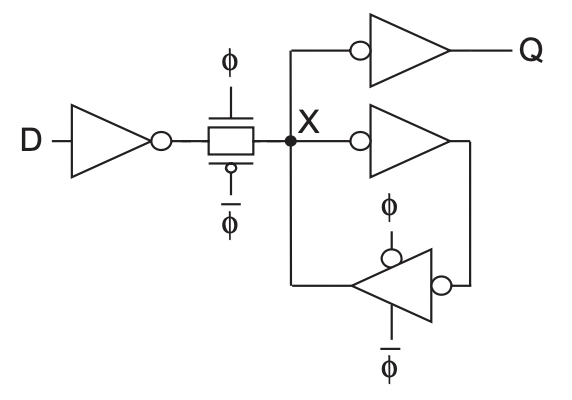
\includegraphics[scale=0.5]{images/static-latch.png}
	\caption{Static Latch}\label{fig:static-latch}
\end{figure}

It has 2 buffers: one for input and one for output. This provides isolation. During the hold stage, $\phi=0$ the tristate inverter is enabled and thus we have the feedback chain storing the value of X. The transmission gate is off which isolates the node X from the D inverter. The output keeps the value of $\overline{X} = \overline{\overline{D}} = D$ and thus we can successfully hold. During the transparent stage, the tristate inverter floats and the transmission gate turns on, allowing $\overline{D}$ to be loaded into $X$ while $Q$ follows as $\overline{X}$ as before.

Note that we can reduce the clock load at the cost of robustness by using a weak inverter instead of a tristate one.

\subsection{Enable and Reset Signals}
An enable signal causes the output to hold when it is off, otherwise allows normal operation. A reset signal forces the output to a 0 when it is raised, otherwise the output is unaffected.

\subsubsection{Enable Signal}
In the MUX design, we may surround a latch with another MUX that feeds the current latch output when EN=0 and otherwise feeds in D. This increases the D to Q delay of the overall latch.

In the clock-gating approach we replace the clock signal with an AND2 over the EN and CLK signal. This adds some skew and increases the setup time of the circuit (the edge takes longer to get to the actual latch).

Synthesis tools generally prefer the MUX design as it doesnt cause clock skew.

\subsubsection{Reset Signal}
A reset may be synchronous or asynchronous. Synchronous resets can by done by replacing the input with an AND2 of D and $\overline{\text{RST}}$. When the reset is high, the and will be forced to 0 and the output will store a 0 on the \textit{next} clock edge.

An asynchronous reset can be acheived by also putting such an AND2 on the inner node that stores the output (or comeplement of the output as in \autoref{fig:static-latch}).

If D is already being inverted (e.g. in \autoref{fig:static-latch}) we can use a NAND2 to do the AND and inversion at the same time.

\subsection{Pulsed and TSPC Latches}

Instead of sequencing logic with flip-flops, we could also use latches and simply give a short pulse to all of them. This is called a \textbf{pulsed} latch and its behaviour is similar to a flip-flop, but generating the pulse while maintining timing is a little trickier.

To generate a pulse we can feed a clock signal into a NAND2 twice, with one path going through $2k+1$ inverters. This causes some overlap between the edges of $\overline{\phi}$ and $\phi$ which will create a regular short pulse from a clock.

A \textbf{True Single-Phase Clock} latch is a clever way of implementing a latch with low clock load. It involves a precharged node and thus the setup/hold time analysis depends on the edge.

\section{Timing}

\subsection{Setup and Hold}\label{sec:setup-hold}
For a latch or flip flop, the \textbf{setup} time is the latest point \textit{before} the clock edge that an input must be stable to ensure that the output gets the correct value. The \textbf{hold} time is the minimum time \textit{after} the clock edge that a signal must be stable for the output to get the correct value. That is, in \autoref{fig:clock-edge-ff}, a signal must be stable for $t \in [t_{\phi2} - t_{setup},\ \ t_{\phi2} + t_{hold}]$ to correctly propagate to the output.

For example, recall the analysis of \autoref{sec:positive-flip-flop}. In that circuit, $x$, the point at which $L_1$ stops following $D_1$ would be related to the setup time as $t_{setup} = t_{\phi2} - x$. The circuit would have \textbf{no hold time} since after $x$ the inner node $Q_1$ is stable and at some point will be output by $L_2$.

\subsection{Clock-to-Q and D-to-Q}\label{sec:cq-dq}
The Clock or D signals have some delay to correspond to a change to the output Q. The D-to-Q value is particularly important in latches since Q may change right after a D change during the transparent state, whereas flip-flops cannot.

The \textbf{minimum} of each of these delays is called the corresponding \textbf{contamination} delay. The \textbf{maximum} of these delays is called the \textbf{propagation} delay.

The contamination and propagation delays can be thought of respectively as the earliest that $Q$ starts 'glitching' and the latest point at which it will stabilize.

\subsection{Logic Delay}\label{sec:logic-delay}
Recall that sequencing elements are there to order the flow of information; that is, they are placed between or at the end of some combinational logic (either FSM or Pipeline as discussed in the section intro). Thus there is also some logic delay with a contamination and propagation value denoted $t_{cd}$ and $t_{pd}$ respectively.

\subsection{Timing Constraints}\label{sec:timing-constraints}
The existence of the timing conditions described in \autoref{sec:setup-hold} combined with the existence of the delays in \autoref{sec:cq-dq} and \autoref{sec:logic-delay} leads to two conditions that must be obeyed for a circuit.

In this section we assume we are working with pipelined flip-flops, thus the \textbf{D-to-Q delay is irrelevant}. Furthermore, we focus on the case of a pair of flip-flops separated by some combinational logic. Call these flip-flops $F_1$ and $F_2$ respectively.

\subsubsection{Maximum Delay Constraints}
This is closely related to the setup time of a latch or flip-flop. Let the period of the clock be T.

When the clock edge arrives at $F_1$, it may or may not cause a change in $Q_1$. If it does not cause a change, then there is nothing to worry about as the combinational logic receives the same input, produces the same output, and thus $D_2$ is stable long before the next clock edge. If it \textit{does} cause a change, it may do so \textbf{as late as} the delay $t_{pcq}$ (propagation clock to Q). The corresponding change in the combinational logic may take as long as $t_{pd}$. Thus the total time from clock edge 1 to $D_2$ is $t_{pcq} + t_{pd}$. This time by definition must be less than the setup time for the next clock edge. This is how we get the \textbf{max-delay constraint} of \autoref{eqn:max-delay-constraint}.

\begin{equation}
	\label{eqn:max-delay-constraint}
	t_{pcq} + t_{pd} \le T - t_{setup}
\end{equation}

Note that since $f = \frac{1}{T}$, \autoref{eqn:max-delay-constraint} gives us the maximum frequency we can run the circuit at, and we can solve this delay simply by slowing down the clock.

\subsubsection{Minimum Delay Constraints}
This is closely related to the hold time of the flip-flop. It is much harder to remedy as T is not a term in the constraint.

A clock transition may cause a $Q_1$ change as soon as $t_{ccq}$. The combinational logic, receiving this change, may cause the value of $D_2$ to change as soon as $t_{cd}$ after. This total time must be \textbf{greater} than the hold time otherwise the data has changed too soon after the clock edge. The constraint is given by \autoref{eqn:min-delay-constraint}.

\begin{equation}
	\label{eqn:min-delay-constraint}
	t_{ccq} + t_{cd} \geq t_{hold}
\end{equation}

The only way to fix this is to redesign the circuit.


\section{Clock Uncertainties}
Ideally, all clock inputs receive the exact same clock signal with period T. In reality, there are many complications that may mess with the clock signal. We consider the two most important: skew - where clock paths have a fixed offset delay relative to eachother, and jitter - where each clock edge may arrive slightly sooner or later than expected in a way that varies over time.

There are many ways to mitigate these issues such as clock H-trees and time borrowing but we do not discuss any of these in detail.

\subsection{Skew}
Skew comes from the layout of each path to the system clock source. Each path may have different RC characteristics and thus each path has a fixed delay relative to each other path. This is \textbf{constant} for a given path and does not affect the period.

The skew $\delta$ for the circuit of \autoref{sec:timing-constraints} is $t_{\phi_2}$ - $t_{\phi_1}$ where $t_{\phi_i}$ is the time at which any clock edge at flip-flop $i$ arrives. Thus it may be positive or negative - each has different implications on the timing constraints of \autoref{sec:timing-constraints}.

\subsubsection{Positive Skew}
If the skew is positive, the clock edge at $F_2$ later than it did at $F_1$. This means that \autoref{eqn:max-delay-constraint} is relaxed since the signal must only arrive at $D_2$ by $T + \delta - t_{setup}$ rather than $T - t_{setup}$. The full constraint is given by \autoref{eqn:skew-max-delay-constraint}.

\begin{equation}
	\label{eqn:skew-max-delay-constraint}
	t_{pd} + t_{pcq} + t_{setup} - \delta \le T
\end{equation}

On the other hand, \autoref{eqn:min-delay-constraint} is worse since we must now hold for $d$ time units longer. The full constraint is given by \autoref{eqn:skew-min-delay-constraint}.

\begin{equation}
	\label{eqn:skew-min-delay-constraint}
	t_{ccq} + t_{cd} \ge t_{hold} + \delta
\end{equation}

\subsubsection{Negative Skew}
This is essentially the inverse of positive skew. It negatively affects the maximum delay constraint because the second clock edge arrives \textit{sooner}. It positively affects the minimum delay because we do not need to hold as long.

The nice thing is that if we simply keep our definition of $\delta$, \autoref{eqn:skew-max-delay-constraint} and \autoref{eqn:skew-min-delay-constraint} still hold for negative skew.

\subsection{Jitter}

Jitter randomly causes edges to arrive sooner or later than usual. The maximum value by which this occurs is $t_{jitter}$. We need to consider the worst case. For maximum delay, the worst case is that $\phi_1$ arrives late and $\phi_2$ arrives early. Adding this to \autoref{eqn:skew-max-delay-constraint} results in \autoref{eqn:skew-jitter-max-delay-constraint}. For minimum delay, the worst case is that $\phi_1$ arrives early and $\phi_2$ arrives late. Adding this to \autoref{eqn:skew-min-delay-constraint} gives \autoref{eqn:skew-jitter-min-delay-constraint}.


\begin{align}
	\label{eqn:skew-jitter-max-delay-constraint}
	t_{pd}+t_{pcq}+t_{setup} &\le T + \delta - 2t_{jitter}\\
	\label{eqn:skew-jitter-min-delay-constraint}
	t_{ccq}+t_{cd} &\ge t_{hold} + \delta + 2t_{jitter}
\end{align}


\chapter{Adders}
Adders are often the speed bottleneck in something like an ALU so it is worth looking at optimizing them heavily. This can occur at the circuit or logic level.

\section{Full Adder}
A full adder takes in bits $A_i, B_i, C_i$ and outputs $C_o, S$ (carry and sum). We can write the functions for the outputs as \autoref{eqn:carry-out} and \autoref{eqn:sum}


\begin{align}
	\label{eqn:carry-out}
	C_o &= AB + C_iA+C_iB = AB + C_i(A+B)\\
	\label{eqn:sum}
	S &= A \oplus B \oplus C_i = \overline{C_o}(A + B + C_i) + ABC_i
\end{align}

Note that $C_i$ arrives later than $A$ and $B$ so it is useful to factor it out and optimize for it (e.g. setting it as the inner input). The value for the sum reuses $\overline{C_o}$ - why? Because the critical path in an adder is the chain of $C_o$ so we might as well reuse it to compute $S$ to reduce the overall area.

The properties \autoref{eqn:inv-sum} and \autoref{eqn:inv-carry} are very important, as they allow us to perform more optimizations.

\begin{align}
	\label{eqn:inv-carry}
	\overline{C_o}(A, B, C_i) &= C_o(\overline{A},\overline{B},\overline{C_i})\\
	\label{eqn:inv-sum}
	\overline{S}(A, B, C_i) &= S(\overline{A},\overline{B},\overline{C_i})
\end{align}

We also define the mutually exclusive \textbf{G}enerate, \textbf{P}ropagate and \textbf{K}ill signals. When the adder generates, its carry out depends only on the bits $A_i$ and $B_i$. When it propagates, its carry out is equal to its carry in independent of $A_i$ and $B_i$. When it kills the carry out is 0.

\begin{align}
	G &= AB \\
	P &= A \oplus B\\
	K &= \overline{A + B}
\end{align}

\section{Ripple Carry-Adder}
To add N bits, we chaing N full adders together. The critical path is the $A$ or $B$ input of bit 0 to the $S$ of bit $N-1$. Thus the overall delay is

\begin{equation}
	\label{eqn:rca-delay}
	t_{add} = (N-1)t_{carry} + t_{sum}
\end{equation}

The circuit involves 3 sections. First, using $A, B, C_i$ we generate $\overline{C_o}$. This value feeds into 2 things: an inverter to generate $C_o$, and the gate that generates $S$.

\section{Inversion}
Given the inversion properties (\autoref{eqn:inv-carry} and \autoref{eqn:inv-sum}) we can improve the worst case delay by removing the inverter that converts the intermediate $\overline{C_o}$ into $C_o$. Bit 0 generates $\overline{C_o}$ (i.e. it doesnt add the inverter) which is fed into bit 1's $C_i$. Bit 1 also inverts the inputs $A_i, B_i$ and thus generates $\overline{C_o(\overline{A_i}, \overline{B_i}, \overline{C_i})} = C_o$. Thus by the inversion properties the output of bit 1 will be $\overline{S_1}$ and $C_{o1}$.

Essentially, every other full-adder takes input $\overline{A_i}, \overline{B_i}$ and generates $\overline{S_i}$ which must then be inverted. This clears the carry-out path of inverters, improving the worst case delay.

\section{Mirror Adder}
A mirror adder is a better structure to implement the inverting adder at the transistor level. We use the form $C_o = (A + B)(C_i + AB)$ to implement the \textbf{PDN} and give the \textbf{PUN} a symmetrical structure. This reduces the transistor stack and thus lets us use narrower transistors, which reduces load capacitance. The $C_i$ bit should also be closest to the output (see \autoref{sec:inner-outer}).

\section{Carry-Bypass Adder}
Carry-bypass adders are used when we have large words to add. We group each $k$ bits together and compute group generate/propagate signals and add a MUX on the output of the block. The MUX takes signal $\prod_i P_i$ to output the block carry in. That is, if all the elements of the block are propagating, we can immediately forward the overall carry in to the output of the block.

If $\prod_i P_i$ is not true, then at least one of the block bits must be the one that generates the carry-out. Thus the worst case path is the time for a carry in in the 0th bit of block 0 to carry to its block output, and then bypass every other block until the end. Once it reaches the last block it must travel through each bit to the end and also factor in $t_{sum}$.

For example, the overall delay for a block size of 4 given N bits is given by \autoref{eqn:carry-bypass-delay}.

\begin{equation}
	\label{eqn:carry-bypass-delay}
	t_{add} = t_{setup} + 4t_{carry} + (N-1)t_{bypass} + (3t_{carry} + t_{sum})
\end{equation}


\chapter{Memory}

\section{RAM Structure}
RAM is an array of N M-bit words. To index them we use a \textbf{row decoder} that takes in $\lg(N)$ 'address bits' and outputs N wordlines. The worldlines are 'one-hot' in that exactly one of them is a 1. The M-bit word is grouped into blocks of $2^K$ bits. Each block outputs all $2^K$ bits accessed by a wordline, which is then MUXed by a $2^K$-to-1 \textbf{column MUX}.

The notation used is that there are L total address bits. K bits go to the column decoder to select each bit of the word. L-K bits go to the row decoder inputs. The dimension of each block is thus $2^{L-K}$ rows by $2^{K}$ columns, for a total cell count of $2^{L-K} \cdot 2^{K} = 2^{L}$. For the overall RAM then, the number of cells/bits is $M\cdot2^{L}$.

To lay out N M-bit words we do the following:
\begin{enumerate}
	\item $L = \lg{N}$
	\item $\text{Rows} = \text{Columns} = \sqrt{MN}$
	\item $K = L - \lg(\text{Rows})$
\end{enumerate}

This is all the information we need to show the widths of everything in the memory structure.

\subsection{Row Decoders}

The wordlines generated by the row decoders are attached to all $M \cdot 2^K$ cells. Thus they may have very high load capacitances so we need to do some design to get a fast access.

\subsubsection{Basic Operation}
Consider the expression for wordline $i$. It consists of a conjunction of the input address bits corresponding to the binary representation of $i$. For example, when $L-K=2$ (4 wordlines):

\begin{align}
	WL_{0} &= \overline{A_3} \ \overline{A_2} \ \overline{A_1} \ \overline{A_0}\\
	WL_{10} &= A_3 \ \overline{A_2} \ A_1 \ \overline{A_0}\\
\end{align}

\subsubsection{Pre-Decoding}
In the previous example, we can observe that one quarter of the wordlines will need the signal $\overline{A_3} \ \overline{A_2}$ while a quarter will use $\overline{A_3} \ A_2$ and so on. Thus to pre-decode we can compute pairwise signals to form a stage which gets fed into NOR. For example:

\begin{align*}
	WL_{3} &= \left(\overline{A_3} \ \overline{A_2}\right) \left(A_1 \ A_2\right) \\
		   &= \overline{ \overline{\overline{A_3} \ \overline{A_2}} + \overline{A_1 \ A_2}} \\
		   &= \text{NOR}(\text{NAND}(\overline{A_3}, \overline{A_2}) + \text{NAND}(A_1, A_2))
\end{align*}

This is just a small example, we can keep adding more pre-decoding levels for higher N.

\subsection{Column MUX}
Essentially we implement a decoder for $2^K$ and feed each of these lines to the gate of an NMOS. These NMOS are connected to the \textbf{bitlines} which all join at the output of the current block. Thus exactly one column is connected to the output at a time.

\subsection{Sense Amplifiers}
At the output of the column blocks we need to amplify any voltage swings using an analog circuit known as a sense amplifier. Essentially a small $\delta{v}$ gets amplified to a full rail-to-rail swing under sufficient conditions.

\section{Memory Cells}
\subsection{SRAM}
Static RAM has a low activity factor, has low density but is very robust. The standard configuration is called 6T SRAM since it uses 6 transistors. The inner cell is a pair of feedback inverters (\autoref{sec:static-latch}) connected to bitlines by \textbf{access transistors}. The access transistors' drains to the bitlines BL and $\overline{\text{BL}}$. The access transistors' gates are connected to the wordline.

Each cell provides 2 access gate capacitances ($2C_g W_{access}$) and 1 drain capacitance on each bitline ($C_dW_{access}$).

\subsubsection{Read Operation}
\begin{enumerate}
	\item BL and $\overline{\text{BL}}$ precharge to $V_{DD}$ (all other bitlines charge to 0)
	\item Turn on the wordline
	\item Current will discharge through one of the inverters' NMOS (the other line will already be high so no current flows)
\end{enumerate}

To ensure that the storage node doesnt float too high during this process, we must ensure that the access transistors are \textbf{weaker} than the inverters' NMOS.

\subsubsection{Write Operation}
\begin{enumerate}
	\item Precharge bitlines
	\begin{itemize}
		\item To write a 1, BL high and $\overline{\text{BL}}$ low
		\item To write a 0, BL low and $\overline{\text{BL}}$ high
	\end{itemize}
	\item Turn on the wordline
	\item One of the nodes will need to discharge through the access transistor while avoiding being pulled up through the PMOS
\end{enumerate}

To ensure that the storage node is overridden, the PMOS must be weaker than the access transistor. \textbf{Note that this includes the mobility factor} and not just the width. If $\mu_n = 2\mu_p$ then equal widths of PMOS and NMOS will satisfy this requirement.
\subsection{DRAM}
Dynamic RAM is higher density, cheaper, less robust, and uses more power. It uses an enhanced source capacitance to store information. This is acheived through a special process which is why memory is manufactured in separate fabs (basically dig a well at the transistor source to increase the capacitances).

\subsubsection{1T DRAM}
Connect the NMOS gate to the wordline and its drain to the bitline. The enhanced capacitance $C_s$ is connected to ground. To read, precharge $\frac{V_{DD}}{2}$ and then connect the bitline. If it is a 0, the bitline will be driven low as charge redistributed between the bitline capacitance and $C_s$. This difference will be amplified by the sense amplifiers.

To write a value, we force the bitline to the desired value and turn on the wordline.

Reads are destructive - this process also moves charge from $C_s$ which may flip the state. Most DRAM is write-after-read to refresh the values (though the latency of the write can be hidden).

\subsubsection{3T DRAM}

\begin{figure}
	\centering
	\begin{circuitikz}
		\draw (0,1) -- +(8, 0) node[right]{WWL} ++(0,-0.5) -- +(8, 0) node[right]{RWL};
		\path (0.5, -2) node(M1)[nmos, rotate=-90]{} node{M1};
		\path (4, -2) node(M2)[nmos]{} node{M2};
		\path (6, -1) node(M3)[nmos, rotate=-90]{} node{M3};
		\draw (M1.G) to[short, -*] (0.5, 1);
		\draw (-1, -1) node[above]{WBL} -- (-1, -3);
		\draw (M1.S) to[short, -*] (-1, -2);
		\draw (M1.D) -- ++(0.5, 0) to[C] +(0, -2) node[ground]{};
		\draw (M1.D) -- (M2.G);
		\draw (M2.D) |- (M3.S);
		\draw (M3.G) to[short, -*] (6, 0.5);
		\draw (M2.S) -- ++(0, -1) node[ground]{};
		\draw (M3.D) to[short, -*] ++(1, 0) -- +(0, 0.5) node[above]{RBL} -- ++(0, -2);
	\end{circuitikz}
	\caption{A 3T DRAM Configuration}\label{fig:3t-dram}
\end{figure}

The ciruit is shown in \autoref{fig:3t-dram}. This is less higher density than 1T DRAM but prevents the destructive read. To write, we precharge the WBL (write bitline) and then turn on the WWL (write wordline). To read, we precharge the RBL to $V_{DD}$ and then turn on the RWL. If the capacitor is charged, M2 will be ON and the output will be driven low - the circuit stores $\overline{X}$. If the capacitor is not charged, the bitline will not change value. The only leakage is through the transistor gate which is fairly low.

\chapter{Integrated Circuit Testing}

The goal is to improve the yield of circuits. It is not unusual to only get a $\sim$80\% yield in modern processes, whereas typical consumer requirements are just 5-50ppm defective. The field of IC testing is vast and is becoming bigger, here we only consider a few basic techniques for validating them.

The error model we assume is that of \textit{stuck-at} faults. There are two types: stuck at 0 or stuck at 1. A stuck-at fault is usually a layout issue and causes a node to be a constant 0 or 1 regardless of the inputs (i.e. it is tied to $V_{DD}$ or GND).

\section{Combinational Logic}\label{sec:combinational-test}
We can design \textbf{test vectors} of input-output pairs that are designed to detect stuck-at faults at particular nodes. Consider the example in \autoref{fig:stuck-at-example}. A common assumption is that there may be at most one stuck-at fault - consider the case of Y being stuck at 1. If we use $(A, B, C, D) = (1, 1, 0, 0)$, then $f = 0$. If Y were stuck at one however, $f$ would be 1. This test vector thus depends on $Y$ \textit{not} being stuck at one - if we run it and it is successful, we know Y is \textit{not} stuck at one. If it fails however, we may not conclude that it is because Y is stuck at one - it could be C or D too.

Using this method we can design $2N$ vectors for an $N$-node circuit to cover all possibilities. This is better than the $2^N$ exhaustive vectors and it comes from the assumption that only one stuck at fault can occur at a time.


\begin{figure}
\centering
	\begin{circuitikz}
		\draw (0,0) node(A)[above]{A} to[short,*-] ++(1,0) node(AND1)[american and port, anchor=in 1]{};
		\draw (AND1.in 2) to[short,-*] ++(-1,0) node[below]{B};

		\draw (0, -2)node(C)[above]{C} to[short, *-] ++(1.5,0) node(OR1)[american or port, anchor=bin 1]{};
		\draw (OR1.bin 2) to[short,-*] ++(-1.5,0) node[below]{D};

		\path (6, -1.5)node(AND2)[american and port]{};
		\draw (AND1.out) -- ++(1,0) node[above]{X} |- (AND2.in 1);
		\draw (OR1.out) -- ++(1,0) node[below]{Y} |- (AND2.in 2);
		\draw (AND2.out) to[short, -*] ++(1,0) node[above]{f};
	\end{circuitikz}
	\caption{Example for Combinational Logic}\label{fig:stuck-at-example}
\end{figure}


\section{Sequential Logic}

The method of \autoref{sec:combinational-test} cannot be used in sequential circuits. The focus here is pipelined circuits (\autoref{sec:sequential-logic}). What we do is design a \textbf{scan chain} by surrounding every flip-flop with a 2-to-1 MUX at its input (known as a \textbf{scan structure}). The MUX is enabled by a 'scan-enable' signal and if it is a 1 the input to the flip-flop comes from the scan-in signal. The scan in signal for a register in a pipeline comes from the output of the previous stage.

Using this, we can manually set the state of $N$ registers in $N$ clock cycles by feeding each bit to the first register.

\end{document}